%%==========================================================================
%% Interview Rosa
%%==========================================================================

\chapter{Interview met Rosa, schooldirectrice}
\label{ch:interviewRosa}

\section{Inleiding}
Carmen Rosa Diaz Fonseca is op dit moment schooldirectrice op een lagere school in Peru. Ze behaalde een postgraduaat in 'gestión pública'. Na haar studies begon ze les te geven in education primaria. Daar gaf ze wiskunde en communicatie aan leerlingen van het lager onderwijs. Daarna ging ze aan de slag bij het ministerie van onderwijs als instructrice om andere leerkrachten op te leiden en als assistent bij UGEL. Dat is een koepel over verschillende scholen per provincie heen. De school waar ze nu werkt heet 'Padre Miguel Marina', en ligt in Jicamarca, in het oosten van Lima. Op dit moment heeft ze meer dan 20 jaar ervaring in de onderwijs sector. Het is interessant om te weten te komen welke kijk ze heeft op informatica in educatie als schooldirectrice en ex-medewerker van het ministerie van onderwijs. Dit interview werd, door de huidige maatregels tegen het Covid-19 virus afgenomen, vanop afstand.

In Figuur \ref{rosa} is Rosa te zien.

\begin{figure}[h!]
	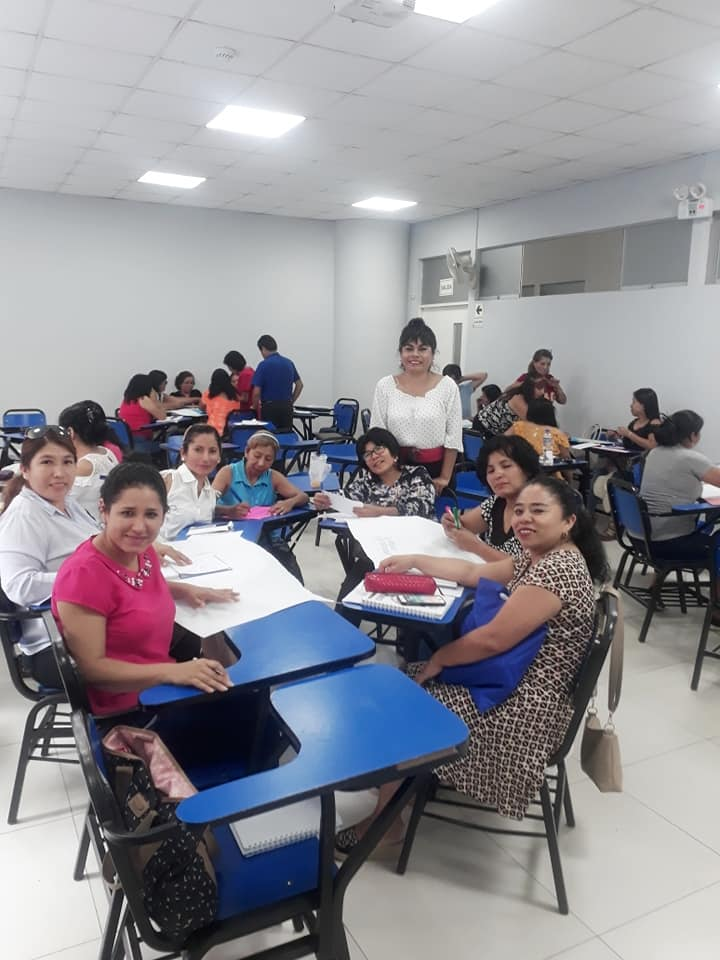
\includegraphics[width=300px]{../img/rosa.jpeg}
	\caption{Rosa Diaz Fonseca (rechtstaand) tijdens een bijles voor leerkrachten }
	\label{rosa}
\end{figure}


\section{Interview}

\textbf{Hoeveel leerlingen zitten er gemiddeld in de klassen waarin u lesgaf?}

\textit{Rosa:} Er zitten volgens mij ongeveer 33 leerlingen in elke klas. Op mijn school zijn er 8 klaslokalen. De volledige school telt ongeveer 265 leerlingen.

\textbf{Hebben de kinderen thuis toegang tot een computer?}

\textit{Rosa:} Peru heeft verschillende klassen. Er is een onderklasse, middenklasse en bovenklasse. De meeste kinderen op mijn school komen vanuit de onderklasse. Die kinderen komen uit arme gezinnen die geen computers ter beschikking hebben. Over het algemeen geldt er dat kinderen uit de middenklasse thuis wel computers hebben.

\textbf{Heeft jouw school computers ter beschikking? Welke apparatuur was er? Zijn er problemen met deze apparatuur?}

\textit{Rosa:} De school heeft 32 computers, maar het zijn geen moderne computers die we normaal gebruiken. Het zijn kleine educatieve computers van het type XO95. Ze zijn wit en groen van kleur. De overheid besliste een aantal jaar geleden om veel geld in het XO project te pompen en veel computers aan te kopen. Ik denk dat ze betere computers met dat geld konden kopen. Het ging toen echt over gigantische bedragen. Op dit moment zijn de computers echt verouderd. Daardoor zijn onbruikbaar. De computerwereld verandert zo snel en onze overheid maakt geen geld vrij om die veranderingen op te volgen.

\textbf{Mogen de kinderen de XO computer meenemen naar huis?}

\textit{Rosa:} Neen, bij ons op school is dat niet de bedoeling. Ik weet dat dat op andere scholen in de binnenstad van Lima wel gebeurd.

\textbf{Als leerlingen informatica les krijgen, wat leren ze dan?}

\textit{Rosa:} De kinderen leren basis dingen zoals schrijven en lezen. De computers worden gebruikt om dat te ondersteunen. Ze zouden gebruikt moeten worden als ondersteuning. In realiteit zijn de computers erg traag. Eigenlijk vangt er weinig mee aan te vangen. Ze zijn erg verouderd.

\textbf{Heeft jouw school een ICT leerkracht?}

\textit{Rosa:} Niet alle scholen hebben informatica leerkrachten. Dit komt omdat de scholen te weinig budget krijgen van het Peruviaanse ministerie van onderwijs en dus de regering. Om die reden hebben wij dus geen leerkracht informatica om die reden. Ik keek er eens voor om een informatica leerkracht op mijn school aan te werven maar dit is gewoonweg onbetaalbaar. Ik verwacht van mijn normale leerkrachten dat ze de taak van informatica leerkracht op zich nemen en de informaticakennis die ze hebben doorgeven aan de kinderen.

\textbf{In hoeverre kunnen uw gewone leerkrachten overweg met informatica?}

\textit{Rosa:} De leerkrachten geven de informatie die ze hebben door aan de leerlingen. Ik weet dat het beter zou zijn moest er een informatica leerkracht zijn, maar die is er niet.

\textbf{Krijgen leerlingen huiswerk op de computer?}

\textit{Rosa:} Ja, de kinderen hebben huiswerk op computers maar maken dat niet thuis. Zoals ik al zei hebben er velen thuis geen computers, en dus gaan ze naar internetcafés. Daar kunnen ze een computer gebruiken om huiswerk op te maken. Echter, in een internetcafé wordt er geen toezicht gehouden op de kinderen. Daarom spelen ze daar vaak spelletjes op de computer en gebruiken ze niet al hun tijd om hun huiswerk te maken. De computers die ze ter beschikking hebben, hebben meestal geen veilig internet voor kinderen. De kinderen zouden per ongelijk op pornografische websites of andere kwaadaardige websites terecht kunnen komen. Daar maak ik me zorgen over.

\textbf{Hoe komt het dat Peru niet verder staat op vlak van informatica, wat liep er fout in het verleden?}

\textit{Rosa:} Eén van de grote problemen in het onderwijs van Peru is het nationale budget dat wordt gespendeerd aan de educatie van kinderen. Volgens mij beseffen ze vaak niet wat de kracht van onderwijs is. 

Daarnaast hebben ongeveer de helft van de scholen geen document dat aantoont dat hun gebouwen eigendom zijn van de staat. Dit zou de overheid in orde moeten brengen. Er is een wet in Peru die voorkomt dat de overheid kan investeren in de infrastucuur en gebouwen van de scholen als de eigendomsrechten niet van de staat zijn. Zelf zorgen er dus voor dat ze geen eigenaar worden van de school zo kunnen ze niet investeren.

Omdat de staat niet investeert verdwijnt er volgens mij veel geld in corruptie. Ze overwaarderen kosten kunnen maar een paar scholen helpen en laten geld verdwijnen. De scholen die ze dan helpen zijn vaak scholen in de hoofdstad waar veel kinderen uit de midden-klasse naar toe gaan. Als scholen niet door de staat gefinancierd worden, gebeurt het dat ouders zelf collectes doen om de school te steunen. De meeste computers op staatsscholen worden aangekocht met steun van ouders die actie ondernamen. 

\textbf{Je gaf ook opleidingen aan leerkrachten. Was er bijles voor informatica?}

\textit{Rosa:} De leerkrachten moeten zichzelf bijscholen op vlak van informatica. We gebruikten tijdens de bijlessen wel computers om filmpjes te kijken of om dia voorstellingen te bekijken, maar echt bijles specifiek voor ICT was er niet. Als een leerkracht bijles informatica wil zal hij daar zelf voor moeten betalen.

\textbf{Heb je op dit moment als directrice zelf geen extra mogelijkheden om de informatica binnen jouw school te verbeteren?}

\textit{Rosa:} We hebben geprobeerd om een programma op te zetten om de informatica op onze school te verbeteren. Dat lukte niet omdat scholen in buitenwijken van de hoofdstad vaak geen basis fundering hebben. Er is geen stroom, licht, stromend water of riolering in deze wijk! Niet alleen scholen hebben te maken met dit probleem ook andere instanties zoals medische posten, die men wil opbouwen in een buitenwijk hebben hiermee te kampen. Mijn school is één van de vele scholen die met dit probleem zit. De overheid zou dit eerst moeten oplossen vooraleer we zelf kunnen denken aan nieuwe computers op school. De huidige XO laptops werken op zonne-energie. 

\textbf{Wat zouden mogelijke oplossingen kunnen zijn voor deze problemen?}

\textit{Rosa:} Ik denk dat de lokale overheden beter zouden moeten functioneren. Als zei de funderingen zouden prioriteren, zouden daar veel mensen en initiatieven mee kunnen geholpen zijn. Ze zouden water, elektriciteit en rioleringen moeten aanleggen. Op dit moment bundelen we de krachten met een aantal lokale instituten om dit toch zelf te kunnen verwezenlijken maar dat is niet simpel. 

Donaties zoeken zou ook kunnen helpen. Ook zouden er activiteiten kunnen georganiseerd worden om geld te verdienen. Ik denk dan aan tombola's of eetfestijnen. Met dat geld zouden er dan computers kunnen aangekocht kunnen worden. ONG's zouden ons ook kunnen helpen. Laatst nog stond ik in contact met een ONG die ons wou helpen met het voorzien van zonne-energie, om zo toch elektriciteit te hebben op onze school.

\subsection{Besluit}
%olpc XO95
Ook op de school van Rosa worden de OLPC XO computers gebruikt. Volgens Rosa pompte Peru veel geld in OLPC. Dat blijkt ook uit de stand van zaken, waar beschreven staat dat in Peru het grootste OLPC programma uitgerold werd. Rosa vertelt ook dat er op haar schol XO95 laptops gebruikt worden. Dat klopt niet. Het type XO95 bestaat niet. Alleen de types XO-1, XO-1.5, XO-1.75, XO-2, XO-3 en XO-4 Touch werden ontworpen. \autocite{OLPC2016}. Nochtans komt haar beschrijving op vlak van de kleuren duidelijk overeen. 

Rosa spreekt ook over een probleem met eigendomsaktes van scholen. In 2004 was 75\% van de scholen in Peru gevestigd in gebouwen die geen wettelijke fysieke sanitaire voorzieningen heeft. Dat komt omdat ze geen eigendomsaktes hebben. Volgens het openbaar register bestaan ze niet. Dit percentage komt overeen met meer dan 31 duizend scholen over heel Peru. Zoals Rosa uitlegt zijn de eigendomsaktes belangrijk om te kunnen investeren in scholen. Als er aanpassingen aan de infrastructuur van een pand of de accommodatie moeten gebeuren, met steun via overheidsgeld, is een eigendomsakte nodig omdat het duidelijk maakt dat de grond geen verplichtingen jegens derden heeft en vrij is van pandrechten. Als dit niet het geval is maakt men geen kans op subsidies, en kan men de scholen niet voorzien van sanitaire voorzieningen.

Het echte probleem is dat de staat niet over de middelen beschikt om deze onderwijsfaciliteiten onmiddellijk te verbeteren. Daarom starten ze weinig procedures op om de eigendomsaktes in orde te brengen. De procedure om eigendomsaktes op te stellen kost trouwens ongeveer 1000 sol(+/- 270 euro) per school. Dat betekent dat er ongeveer 31 duizend sol (+/-8,4 miljoen euro) nodig is om de eigendomsaktes van de overige 75\% van de scholen in orden te brengen. Volgens overheid gaat dit om te veel geld dat ze beter op andere manieren kunnen investeren. \autocite{larepublica2004}
